% !TeX program = xelatex
% 编译：xelatex main.tex（连跑两次，第一次生成目录/引用，第二次解析）
\def\allfiles{}   % 标记：篇章文件被主文件包含时不再重复加载导言区
\documentclass[12pt, a4paper, oneside, UTF8]{ctexbook}
\usepackage{xcolor}                  % personal.tex 中要先定义颜色，故提前加载
% =============================================================
%  个人配置文件  ——  ★ 每次写新笔记，通常只改这个文件 ★
%  所有"专属于你"的内容都集中在这里，正文章节保持干净。
% =============================================================

% ---------- 0. 语言开关（★ 一键切换中英文）----------
% 默认中文版；把下一行改成 \Englishtrue 即整体切换为英文版。
% 作用范围：封面、前言、定理/证明等环境名、括号、章节标题、目录名、日期。
% 注意：章节正文需自己写成对应语言，开关不会翻译正文内容。
\newif\ifEnglish
\Englishfalse      % \Englishfalse = 中文版   |   \Englishtrue = 英文版

% ---------- 1. 封面与前言（中英各一套）----------
\ifEnglish
  \def\myTitle{Math Notes}
  \def\mySubtitle{Analysis · Review and Synthesis}
  \def\myAuthor{Your Name}
  \def\myCourse{Course / Class}
  \def\myTerm{Academic Year 2026}
  \def\engToday{%
    \ifcase\month\or January\or February\or March\or April\or May\or June\or
    July\or August\or September\or October\or November\or December\fi\ \the\day,\ \the\year}
  \def\myDateCover{\engToday}
  \def\myForeword{Preface}
  \def\myForewordText{
    This is your personal \LaTeX{} template for math notes: theorems, lemmas,
    corollaries and criteria share one numbering sequence; definitions, propositions
    and examples are numbered independently; remarks, proofs and solutions are
    unnumbered.\par
    \medskip
    Just maintain the chapter files under \texttt{chapters/}; to change the title,
    author, colors or theorem names, edit this \texttt{personal.tex} only.
  }
\else
  \def\myTitle{数学笔记}
  \def\mySubtitle{数学分析 · 复习与整理}
  \def\myAuthor{你的名字}
  \def\myCourse{课程 / 班级}
  \def\myTerm{2026 学年}
  \def\myDateCover{\today}
  \def\myForeword{使用说明}
  \def\myForewordText{
    这是一份属于你自己的数学笔记模板：定理、引理、推论、准则共用一套编号；
    定义、命题、例题各自编号；注、证明、解不编号。\par
    \medskip
    写作时只需维护 \texttt{chapters/} 下的章节文件；
    修改标题、作者、配色、定理名称，只改本文件 \texttt{personal.tex} 即可。
  }
\fi

% ---------- 2. 主题配色（整套换色只改这里）----------
% 数字为 RGB 十六进制；主色用于页眉、链接、封面装饰
\definecolor{themeMain}{HTML}{2B5F8A}      % 主色（深蓝）
\definecolor{themeAccent}{HTML}{C0563B}    % 强调色（砖红）

% ============================================================
%  5 大核心色系：8 个环境合并为 5 色，以"同色不同形"区分主次
%  （本处只定义颜色；盒子的边框/底色分级见 config/theorems.tex）
% ------------------------------------------------------------
%  绿色系 → 定义（基础、自然）
%  蓝色系 → 定理 / 命题 / 准则（冷静、理性）
%           定理：实心浅蓝底；命题、准则：极浅蓝底 + 0.4pt 细外框
%  紫色系 → 推论 / 引理（知识、派生）
%           推论：浅紫底；引理：白底 + 0.4pt 紫色细外框
%  米灰系 → 例题（低饱和、低调）：白底 + 2.5pt 左竖线，长例题不染花页面
%  砖红系 → 注释（警觉、强调）
% ============================================================
% 1. 绿色系：定义
\definecolor{defMain}{HTML}{2E8B57}
\definecolor{defBg}{HTML}{EAF6EE}
% 2. 蓝色系：定理 / 命题 / 准则
\definecolor{thmMain}{HTML}{2B6FA8}
\definecolor{thmBg}{HTML}{E8F1FB}      % 定理专用：实心浅蓝底
\definecolor{propBg}{HTML}{F6FAFE}     % 命题/准则专用：极浅蓝底
% 3. 紫色系：推论 / 引理
\definecolor{corMain}{HTML}{7D5BA6}
\definecolor{corBg}{HTML}{F1ECFA}      % 推论专用：浅紫底
% 4. 中性米灰：例题
\definecolor{exMain}{HTML}{7A7568}     % 加深的米灰，解决标题发灰问题
\definecolor{exBg}{HTML}{F8F7F4}       % 备用浅米底（默认使用纯白底留白）
% 5. 砖红系：注释/注记
\definecolor{remMain}{HTML}{B54848}
\definecolor{remBg}{HTML}{FBEDED}

% ---------- 3. 定理环境的显示名称与括号（中英各一套）----------
% 想单独改某个词，改对应分支里的中文或英文即可。
\ifEnglish
  \def\nmDef{Definition}
  \def\nmThm{Theorem}
  \def\nmLemma{Lemma}
  \def\nmCor{Corollary}
  \def\nmCri{Criterion}
  \def\nmPro{Proposition}
  \def\nmRmk{Remark}
  \def\nmEx{Example}
  \def\nmProof{Proof}
  \def\nmSol{Solution}
  \def\nmLParen{(}
  \def\nmRParen{)}
\else
  \def\nmDef{定义}
  \def\nmThm{定理}
  \def\nmLemma{引理}
  \def\nmCor{推论}
  \def\nmCri{准则}
  \def\nmPro{命题}
  \def\nmRmk{注释}
  \def\nmEx{例}
  \def\nmProof{证明}
  \def\nmSol{解}
  \def\nmLParen{（}
  \def\nmRParen{）}
\fi

% ---------- 4. 章节标题 / 目录名（随语言切换）----------
\ifEnglish
  \ctexset{
    chapter/name = {Chapter\space},
    chapter/number = \arabic{chapter},
    chapter/aftername = \space,
  }
  \renewcommand{\contentsname}{Contents}
\fi
                     % 唯一个人配置文件：改标题/姓名/配色就改它
% 宏包与全局排版设置（一般不需要改）

\usepackage{amsmath, amssymb, amsthm, mathtools}
\usepackage{graphicx}
\usepackage{geometry}
\usepackage{enumitem}
\usepackage{fancyhdr}
\usepackage{listings}
\usepackage{esint}
\usepackage{mathrsfs}
\usepackage{extarrows}
\usepackage{stackengine}
\usepackage{booktabs}
\usepackage[most]{tcolorbox}
\usepackage[colorlinks=true, linkcolor=themeMain, citecolor=themeMain,
            urlcolor=themeMain, breaklinks=true]{hyperref}

% 图片统一放 figures/，正文里写文件名即可，无需带路径
\graphicspath{{figures/}, {../figures/}, {../../figures/}}

% 页面布局：A4、1.45 倍行距，适合长时间阅读与手写批注
\linespread{1.45}
\geometry{
  top=25mm, bottom=23mm, left=22mm, right=22mm,
  headheight=14pt, headsep=5mm, footskip=11mm
}

% 列表间距收紧一点，笔记更紧凑
\setenumerate[1]{itemsep=3pt, partopsep=0pt, parsep=2pt, topsep=4pt}
\setitemize[1]{itemsep=3pt, partopsep=0pt, parsep=2pt, topsep=4pt}
\setdescription{itemsep=3pt, partopsep=0pt, parsep=2pt, topsep=4pt}

% 页眉页脚：左章名、右节名、居中页码
\pagestyle{fancy}
\fancyhf{}
\fancyhead[L]{\small\color{themeMain!80!black}\nouppercase{\leftmark}}
\fancyhead[R]{\small\color{themeMain!80!black}\nouppercase{\rightmark}}
\fancyfoot[C]{\thepage}
\renewcommand{\headrulewidth}{0.4pt}
\renewcommand{\footrulewidth}{0pt}

% 代码/符号环境样式（LaTeX 源码与 Mathematica）
\lstset{
  basicstyle=\ttfamily\small, breaklines=true, columns=flexible,
  keywordstyle=\bfseries\color{themeMain}, commentstyle=\itshape\color{black!55},
  stringstyle=\color{themeAccent}, numbers=left, numberstyle=\footnotesize,
  frame=tb, xleftmargin=1.2em,
}

% =============================================================
%  数学快捷命令库  ——  写公式时少敲键盘
%  用法速查见 README.md；新增自己的命令直接追加到文件末尾。
% =============================================================

% ---------- 数集 ----------
\newcommand{\R}{\mathbb{R}}   % 实数集
\newcommand{\Z}{\mathbb{Z}}   % 整数集
\newcommand{\N}{\mathbb{N}}   % 自然数集
\newcommand{\Q}{\mathbb{Q}}   % 有理数集
\newcommand{\C}{\mathbb{C}}   % 复数集

% ---------- 微分与向量 ----------
\renewcommand{\d}{\mathrm{d}}                       % 微分号 d（ upright）
\newcommand{\pd}[2]{\frac{\partial #1}{\partial #2}} % 偏导 \pd{f}{x}
\newcommand{\bs}[1]{\boldsymbol{#1}}                % 加粗：向量/矩阵
\newcommand{\ora}[1]{\overrightarrow{#1}}           % 箭头：\ora{AB}
\newcommand{\grad}{\nabla}                          % 梯度
\newcommand{\dive}{\operatorname{div}}              % 散度
\newcommand{\rotn}{\operatorname{rot}}              % 旋度
\newcommand{\curl}{\operatorname{curl}}             % 旋度（另一写法）

% ---------- 常用运算符 ----------
\newcommand{\rank}{\operatorname{rank}}
\newcommand{\diag}{\operatorname{diag}}
\newcommand{\tr}{\operatorname{tr}}
\newcommand{\dist}{\operatorname{dist}}
\newcommand{\sgn}{\operatorname{sgn}}
\newcommand{\Var}{\operatorname{Var}}
\newcommand{\Cov}{\operatorname{Cov}}
\newcommand{\argmax}{\operatorname*{arg\,max}}
\newcommand{\argmin}{\operatorname*{arg\,min}}
\newcommand{\esssup}{\operatorname*{ess\,sup}}
\newcommand{\ceil}[1]{\left\lceil #1 \right\rceil}
\newcommand{\floor}[1]{\left\lfloor #1 \right\rfloor}
\newcommand{\abs}[1]{\left\lvert #1 \right\rvert}
\newcommand{\norm}[1]{\left\lVert #1 \right\rVert}
\newcommand{\inner}[2]{\left\langle #1,#2 \right\rangle}
\newcommand{\T}{\mathsf{T}}                         % 转置 A^{\T}

% ---------- 关系与记号 ----------
\newcommand{\defeq}{\coloneqq}                      % 定义为
\newcommand{\pll}{\;\/\!/\:}                        % 平行符号
\newcommand{\ind}[1]{\mathbf{1}_{#1}}               % 示性函数
\newcommand{\dx}[1]{\d #1}                          % \dx{x} -> dx

% ---------- 排版辅助 ----------
\newcommand{\myspace}[1]{\par\vspace{#1\baselineskip}}   % 空 n 行
\newcommand{\tabincell}[2]{\begin{tabular}{@{}#1@{}}#2\end{tabular}} % 表格内换行
\newcommand{\xrowht}[1][12pt]{\rule{0pt}{#1}} % 加高表格行：\xrowht[20pt]

% ---------- 常用环境（可带行高参数）----------
\newenvironment{ca}[1][1]{\linespread{#1}\selectfont\begin{cases}}{\end{cases}}
\newenvironment{vx}[1][1]{\linespread{#1}\selectfont\begin{vmatrix}}{\end{vmatrix}}
\newenvironment{pmat}[1][1]{\linespread{#1}\selectfont\begin{pmatrix}}{\end{pmatrix}}
\newenvironment{bmat}[1][1]{\linespread{#1}\selectfont\begin{bmatrix}}{\end{bmatrix}}

% ---------- 便捷书写 ----------
\newcommand{\todo}[1]{\textcolor{themeAccent}{【#1】}}  % 待办/重点提醒
\newcommand{\note}[1]{\marginpar{\scriptsize\color{themeMain}#1}} % 页边批注

% =============================================================
%  彩色定理环境（tcolorbox 实现）
%  编号规则：定义单独编号；定理/引理/推论/准则共用编号；
%            命题、例题各自编号；注、证明、解不编号。
%  配色：5 大色系 + "同色不同形"三级样式，颜色定义在 personal.tex
%  相比旧版 framed 方案：可跨页、框内可放图片，样式更稳。
% =============================================================

% ---------- 计数器 ----------
\newcounter{Def}[section]
\renewcommand{\theDef}{\thesection.\arabic{Def}}
\newcounter{noteThm}[section]
\renewcommand{\thenoteThm}{\thesection.\arabic{noteThm}}
\newcounter{Pro}[section]
\renewcommand{\thePro}{\thesection.\arabic{Pro}}
\newcounter{Ex}[section]
\renewcommand{\theEx}{\thesection.\arabic{Ex}}

% ---------- 基础样式 ----------
\tcbset{
  mathboxbase/.style={
    enhanced, breakable,
    arc=2pt,
    boxrule=0pt, leftrule=3pt,
    left=8pt, right=8pt, top=6pt, bottom=6pt,
    fonttitle=\bfseries,
    attach title to upper={\par\vspace{3pt}},
    before skip=7pt, after skip=7pt,
  }
}

% 【第一层级：实心浅底】定义、定理、推论、注释
\tcbset{
  defstyle/.style={mathboxbase, colframe=defMain, colback=defBg, coltitle=defMain},
  thmstyle/.style={mathboxbase, colframe=thmMain, colback=thmBg, coltitle=thmMain},
  corstyle/.style={mathboxbase, colframe=corMain, colback=corBg, coltitle=corMain},
  remstyle/.style={mathboxbase, colframe=remMain, colback=remBg, coltitle=remMain},
}

% 【第二层级：浅底/白底 + 0.4pt 细外框】命题、准则、引理（同色不同形）
\tcbset{
  propstyle/.style={mathboxbase, colframe=thmMain, colback=propBg, coltitle=thmMain,
    toprule=0.4pt, bottomrule=0.4pt, rightrule=0.4pt},
  critstyle/.style={mathboxbase, colframe=thmMain, colback=propBg, coltitle=thmMain,
    toprule=0.4pt, bottomrule=0.4pt, rightrule=0.4pt},
  lemstyle/.style={mathboxbase, colframe=corMain, colback=white, coltitle=corMain,
    toprule=0.4pt, bottomrule=0.4pt, rightrule=0.4pt},
}

% 【第三层级：无底色留白 + 2.5pt 左竖线】例题（高频长篇幅，避免染花页面）
\tcbset{
  exstyle/.style={mathboxbase, colframe=exMain, colback=white, coltitle=exMain,
    leftrule=2.5pt, toprule=0pt, bottomrule=0pt, rightrule=0pt},
}

% ---------- 环境定义 ----------
\newtcolorbox{definition}[1][]{
  defstyle,
  code={\refstepcounter{Def}},
  title={\nmDef~\theDef\ifstrempty{#1}{}{\nmLParen#1\nmRParen}}
}

\newtcolorbox{theorem}[1][]{
  thmstyle,
  code={\refstepcounter{noteThm}},
  title={\nmThm~\thenoteThm\ifstrempty{#1}{}{\nmLParen#1\nmRParen}}
}

\newtcolorbox{lemma}[1][]{
  lemstyle,
  code={\refstepcounter{noteThm}},
  title={\nmLemma~\thenoteThm\ifstrempty{#1}{}{\nmLParen#1\nmRParen}}
}

\newtcolorbox{corollary}[1][]{
  corstyle,
  code={\refstepcounter{noteThm}},
  title={\nmCor~\thenoteThm\ifstrempty{#1}{}{\nmLParen#1\nmRParen}}
}

\newtcolorbox{criterion}[1][]{
  critstyle,
  code={\refstepcounter{noteThm}},
  title={\nmCri~\thenoteThm\ifstrempty{#1}{}{\nmLParen#1\nmRParen}}
}

\newtcolorbox{proposition}[1][]{
  propstyle,
  code={\refstepcounter{Pro}},
  title={\nmPro~\thePro\ifstrempty{#1}{}{\nmLParen#1\nmRParen}}
}

\newtcolorbox{remark}[1][]{
  remstyle,
  title={\nmRmk\ifstrempty{#1}{}{\nmLParen#1\nmRParen}}
}

\newtcolorbox{example}[1][]{
  exstyle,
  code={\refstepcounter{Ex}},
  title={\nmEx~\theEx\ifstrempty{#1}{}{\nmLParen#1\nmRParen}}
}

% ---------- 证明 / 解（不编号，颜色统一指向蓝色系主色）----------
\renewcommand{\proofname}{\indent\textbf{\textcolor{thmMain}{\nmProof}}}
\newenvironment{solution}
  {\begin{proof}[\indent\textbf{\textcolor{thmMain}{\nmSol}}]}
  {\end{proof}}


\begin{document}
% 封面 + 前言 + 目录 + 正文页码初始化

% ---------- 封面 ----------
\begin{titlepage}
\thispagestyle{empty}
\centering
\vspace*{3cm}
{\color{themeMain}\rule{\linewidth}{1.2pt}}
\vspace{0.8cm}
{\Huge\bfseries \myTitle\par}
\vspace{0.3cm}
{\Large\color{themeMain} \mySubtitle\par}
\vspace{0.2cm}
{\color{themeMain}\rule{\linewidth}{1.2pt}}
\vfill
{\large \myAuthor\par}
\vspace{0.3cm}
{\normalsize \myCourse \quad \myTerm\par}
\vspace{0.2cm}
{\normalsize \myDateCover\par}
\vspace*{2cm}
\end{titlepage}

% ---------- 前言 ----------
\newpage
\thispagestyle{empty}
\begin{center}
  {\Huge\textbf{\myForeword}}
\end{center}
\vspace{1cm}
\myForewordText
\vfill
\begin{flushright}
  \myDateCover
\end{flushright}

% ---------- 目录 ----------
\newpage
\pagestyle{plain}
\pagenumbering{Roman}
\setcounter{page}{1}
\tableofcontents

% ---------- 正文 ----------
\newpage
\pagenumbering{arabic}
\setcounter{chapter}{0}
\setcounter{page}{1}
\pagestyle{fancy}


% 章节模板：本文件既可随 main.tex 整体编译，也可在此目录单独 xelatex chap.tex
\ifx\allfiles\undefined
\documentclass[12pt, a4paper, oneside, UTF8]{ctexbook}
\usepackage{xcolor}
\input{../../personal}
\input{../../config/packages}
\input{../../config/mathmacros}
\input{../../config/theorems}
\begin{document}
\else
\fi

\chapter{极限与连续}

本章演示模板的核心功能：彩色定理框、数学快捷命令、表格与图片。
所有编号、页眉页脚与目录均自动生成。

\section{映射与函数}

\begin{definition}[映射]
  设 $X,Y$ 是两个非空集合。若存在对应法则 $f$，使得对 $X$ 中每个元素 $x$，
  在 $Y$ 中都有唯一确定的元素 $y$ 与之对应，则称 $f$ 为从 $X$ 到 $Y$ 的\textbf{映射}，
  记作 $f:X\to Y$，其中 $y=f(x)$。
\end{definition}

\begin{remark}
  \todo{注意} 映射要求"每个 $x$ 恰有一个像"，但允许不同的 $x$ 对应同一个 $y$。
\end{remark}

\section{极限的定义}

\begin{definition}[数列极限]
  设 $\{a_n\}$ 为一数列，$A\in\R$。若对任意 $\varepsilon>0$，存在正整数 $N$，
  使得当 $n>N$ 时恒有 $\abs{a_n-A}<\varepsilon$，则称数列 $\{a_n\}$ \textbf{收敛于} $A$，
  记作 $\lim\limits_{n\to\infty}a_n=A$。
\end{definition}

\begin{theorem}[夹逼准则]
  若数列 $\{a_n\},\{b_n\},\{c_n\}$ 满足
  \[
    a_n\le b_n\le c_n \quad (n=1,2,\dots),
  \]
  且 $\lim\limits_{n\to\infty}a_n=\lim\limits_{n\to\infty}c_n=A$，
  则 $\lim\limits_{n\to\infty}b_n=A$。\label{thm:squeeze}
\end{theorem}

\begin{proof}
  对任意 $\varepsilon>0$，由 $\lim a_n=A$ 知存在 $N_1$，当 $n>N_1$ 时 $A-\varepsilon<a_n$；
  由 $\lim c_n=A$ 知存在 $N_2$，当 $n>N_2$ 时 $c_n<A+\varepsilon$。
  取 $N=\max\{N_1,N_2\}$，则当 $n>N$ 时
  \[
    A-\varepsilon<a_n\le b_n\le c_n<A+\varepsilon,
  \]
  即 $\abs{b_n-A}<\varepsilon$，故 $\lim b_n=A$。\qedhere
\end{proof}

\begin{corollary}
  若 $\abs{b_n}\le c_n$ 且 $\lim c_n=0$，则 $\lim b_n=0$。
\end{corollary}

\begin{proposition}[有界性与收敛性]
  收敛数列必有界；但有界数列不一定收敛，例如 $a_n=(-1)^n$。
\end{proposition}

\section{常用记号速查}

下面是本模板内置快捷命令的实际排版效果，写笔记时可以直接调用。

\begin{example}[快捷命令]
  数集：$\R,\Z,\N,\Q,\C$；\quad 向量：$\bs{x}$，$\ora{AB}$；\quad
  微分：$\d x$，偏导：$\pd{f}{x}$；\quad 梯度散度：$\grad f,\ \dive \bs{F},\ \curl \bs{A}$。
  \par 运算符：$\rank A,\ \diag(a_1,a_2),\ \norm{x},\ \abs{x},\ \inner{f}{g},\ A^{\T}$。
\end{example}

\begin{example}[分段与矩阵]
  \[
    f(x)=\begin{ca}
      x^2, & x\ge 0\\
      -x,  & x<0
    \end{ca},
    \qquad
    \bs{A}=\begin{pmat}
      1 & 2\\
      3 & 4
    \end{pmat}.
  \]
\end{example}

\begin{table}[htbp]
  \centering
  \caption{无穷小的比较（\texttt{xrowht} 加高行距示意）}
  \begin{tabular}{@{}ll@{}}
    \toprule
    关系 & 定义 \\
    \midrule\hline\xrowht[20pt]
    $\alpha\sim\beta$ & $\lim \alpha/\beta=1$ \\
    \hline\xrowht[20pt]
    $\alpha=o(\beta)$ & $\lim \alpha/\beta=0$ \\
    \bottomrule
  \end{tabular}
\end{table}

\section{图文混排}

图 1 展示了一个简单函数图像。图片统一放入 \texttt{figures/} 目录，
正文里只需写文件名；定理框内也可以放图片。

\begin{figure}[htbp]
  \centering
  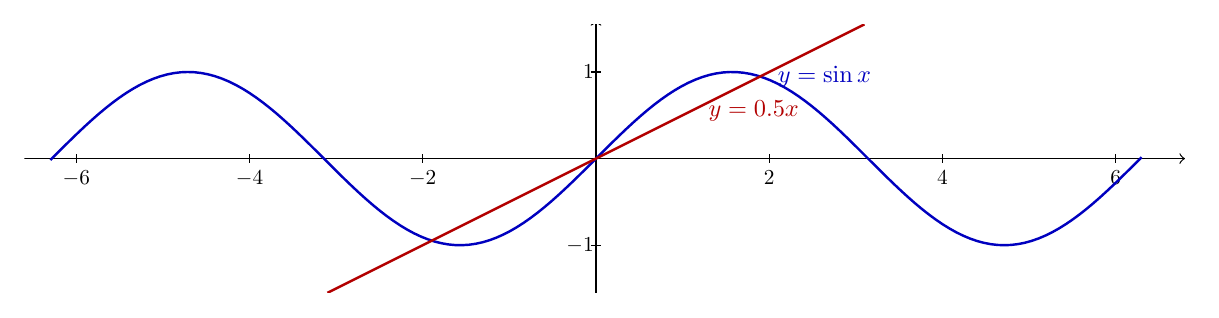
\includegraphics[width=0.62\linewidth]{example-curve.png}
  \caption{函数 $y=\sin x$ 与 $y=0.5x$ 的图像}
\end{figure}

\begin{lemma}[局部有界性]
  若函数 $f$ 在 $x_0$ 处连续，则 $f$ 在 $x_0$ 的某邻域内有界。
\end{lemma}

\begin{criterion}[柯西收敛准则]
  数列 $\{a_n\}$ 收敛的充要条件是：对任意 $\varepsilon>0$，存在 $N$，
  当 $m,n>N$ 时恒有 $\abs{a_m-a_n}<\varepsilon$。
\end{criterion}

\begin{solution}
  这里演示 \texttt{solution} 环境（不编号，标题为"解"）。
  \todo{提示} 用 \texttt{todo} 命令插入醒目的重点提醒。
  \note{页边批注示例}
\end{solution}

\ifx\allfiles\undefined
\end{document}
\fi

% 写自己的笔记：复制 chapters/00-template/chap.tex 到新文件夹，然后取消下一行注释
% % 空白章节模板：复制到新文件夹后，把 {{章节标题}} 换成实际标题即可写作。
% 本文件既可随 main.tex 整体编译，也可在本目录单独 xelatex chap.tex 预览。
\ifx\allfiles\undefined
\documentclass[12pt, a4paper, oneside, UTF8]{ctexbook}
\usepackage{xcolor}
\input{../../personal}
\input{../../config/packages}
\input{../../config/mathmacros}
\input{../../config/theorems}
\begin{document}
\else
\fi

\chapter{{{章节标题}}}

\section{第一节}

在这里写正文。常用环境示例：

% 取消注释即可使用（按需删掉不用的）：
% \begin{definition}[名称] ... \end{definition}
% \begin{theorem}[名称] ... \end{theorem}
% \begin{lemma} ... \end{lemma}
% \begin{corollary} ... \end{corollary}
% \begin{criterion} ... \end{criterion}
% \begin{proposition} ... \end{proposition}
% \begin{remark} ... \end{remark}
% \begin{example} ... \end{example}
% \begin{proof} ... \end{proof}
% \begin{solution} ... \end{solution}

% 图片放在 figures/ 目录：
% \begin{figure}[htbp]\centering
%   \includegraphics[width=0.7\linewidth]{your-figure.png}
%   \caption{图注}\label{fig:xxx}
% \end{figure}

% 公式：
% \begin{equation}\label{eq:xxx} f(x) = \dots \end{equation}

\ifx\allfiles\undefined
\end{document}
\fi


\end{document}
